% * * * * * * * * * * * * * * * * * * * * * * * * * * * * * * * * * * * * * * *
% * * * * * * * * * * * * * * * * * ENTETE  * * * * * * * * * * * * * * * * * *
% * * * * * * * * * * * * * * * * * * * * * * * * * * * * * * * * * * * * * * *

\documentclass[9pt]{beamer}



% * * * * * * * * * * * * * * PACKAGES CLASSIQUES * * * * * * * * * * * * * * *
\usepackage[T1]{fontenc} 
\usepackage[utf8]{inputenc}
\usepackage[frenchb]{babel}
\usepackage{amsmath}
\usepackage{xcolor}  
\usepackage{graphicx}
\usepackage{tikz}
\usepackage{xmpmulti}
%\usepackage{bibentry}										% Bibentry in footnote for example
%\usepackage{inlinebib}
%\nobibliography*
%\usepackage{natbib}										% Reimplement the LATEX \cite command

% * * * * * * * * * * * * * * *  ANIMATIONS * * * * * * * * * * * * * * * * * *
\usepackage{animate}

% * * * * * * * * * * * * * * CHOIX DU THEME  * * * * * * * * * * * * * * * * *
\usepackage{beamerthemeFrankfurt}                                % un theme voir .../beamer/theme/

% * * * * * * * * * * * * * LA BARRE DE NAVIGATION  * * * * * * * * * * * * * *
% commenter la ligne pour supprimer un éléments
\setbeamertemplate{navigation symbols}{%
%	\insertslidenavigationsymbol%
%	\insertframenavigationsymbol%
%	\insertsubsectionnavigationsymbol%
%	\insertsectionnavigationsymbol%
%	\insertdocnavigationsymbol%
%	\insertbackfindforwardnavigationsymbol%
}

% * * * * * * * * * * * * * * * * * TEXTPOS * * * * * * * * * * * * * * * * * *
\usepackage[absolute,showboxes,overlay]{textpos}
\TPshowboxestrue                                              % affiche le contour des textblocks
\TPshowboxesfalse                                             % fait disparaitre le contour des textblocks
\textblockorigin{2mm}{8mm}                                    % origine des positions pour placer les textblocks

% * * * * * * * * * * * * * * * * * PICTURE * * * * * * * * * * * * * * * * * *
\usepackage{picture}
\setlength{\unitlength}{1mm}                                  % définition de l'unité

% * * * * * * * * * * * * * * *  LES BLOCKS * * * * * * * * * * * * * * * * * *
\setbeamertemplate{blocks}[rounded][shadow=true]              % pour des blocks arrondis
\setbeamercolor{block body alerted}{fg=white,bg=monred}       % ecrit en blanc sur fond rouge
\setbeamercolor{block body}{fg=white,bg=monbleu}              % ecrit en blanc sur fond bleu

% * * * * * * * * * * * * * DETAILS DE STYLE  * * * * * * * * * * * * * * * * *
\beamertemplatetransparentcovered                             % Fait afficher l'ensemble du frame en peu lisible (gris clair) dès l'ouverture

\setbeamertemplate{itemize item}[ball]                        % style item
\setbeamertemplate{itemize subitem}[triangle]                 % style subitem
\setbeamertemplate{footline}[page number]
%\setbeamertemplate{footline}[text line]{\href{http://www.christophe-rigaud.com}{Christophe Rigaud}}
  %\vspace*{-1cm}\centering\normalsize Some information\\[0.3em] some more info\\[0.3em]} 
  
%\logo{
\includegraphics[height=5mm]{image/lisa.png}}           % définition du logo 

\renewcommand{\arraystretch}{1.4}                             % espacement des cellules du tableau 

\definecolor{monred}{HTML}{9D0909}                            % un rouge
\definecolor{monbleu}{HTML}{000066}                           % un bleu
\definecolor{monvert}{HTML}{00AE00}                           % un vert

%\renewcommand{\footnoterule}{}                                % supprime le trait au dessus des footnotes
%\renewcommand{\thefootnote}{\alph{footnote}}                  % numérotation par des lettres

% * * * * * * * * * * * * * *  PAGES DE TITRE * * * * * * * * * * * * * * * * *
\title[Abbrev. Title\hspace{2em}\insertframenumber/\inserttotalframenumber]{Image interpretation and conceptual graph integrating topologic and photometric knowledge}
%\subtitle{Application to synthetic image thresholding and medical image windowing}
\author[CR]{\href{http://www.christophe-rigaud.com}{Christophe RIGAUD}}
\institute{LABORATOIRE D’INGÉNIERIE DES SYSTÈMES AUTOMATISÉS}
\date{ 7 July 2011 }

% * * * * * * * * * * * * * * * *  SOMMAIRE * * * * * * * * * * * * * * * * *
\AtBeginSection[]{
  \begin{frame}{Road map}
  \small \tableofcontents[currentsection, hideothersubsections]
  \end{frame} 
}
% * * * * * * * * * * * * * PARAMETRES POUR PDF * * * * * * * * * * * * * * * *
\hypersetup{% Modifiez la valeur des champs suivants
	pdfauthor   = {Christophe Rigaud},%
	pdftitle    = {Titre},%
	pdfsubject  = {Sujet},%
	pdfkeywords = {Mots clés},%
	pdfcreator  = {PDFLaTeX},%
	pdfproducer = {PDFLaTeX},%
	%pdfpagemode = {FullScreen}%                           % ouvre le pdf directement en plein écran
}



% * * * * * * * * * * * * * * * * * * * * * * * * * * * * * * * * * * * * * * *
% * * * * * * * * * * * * * *  DEBUT DOCUMENT * * * * * * * * * * * * * * * * *
% * * * * * * * * * * * * * * * * * * * * * * * * * * * * * * * * * * * * * * *

\begin{document}
	\definecolor{MyGreen}{rgb}{0.0,0.5,0.0}
	%%clear; bibtex main.aux;pdflatex main.tex;evince main.pdf &

%Vous préparerez un exposé de 25 minutes qui sera suivi d'une séance de questions.
%Au cours de l'exposé vous devrez :
%1. Formuler un rappel bibliographique et la problématique qui vous a été proposée. -> problem statement + bilio
%2. Présenter les solutions explorées, et les solutions proposées. -> to do list + explanations
%3. Préciser l'originalité de votre travail par rapport à l'existant. Mix photo + topo -> 3D -> liver -> histo -> threshold -> ident -> vessel
%4. Montrer les résultats obtenus et préciser votre apport. -> quantitative analysis
%5. Préciser les publications envisagées. -> possible

% * * * * * * * * * * * * * * * * * * * * * * * * * * * * * * * * * * * * * * * Slide


\begin{frame}
	\center Soutenance de Master Recherche Mathématiques et Applications
	\center Spécialité : Systèmes Dynamiques et Signaux\vspace{2em}
	\titlepage
	\thispagestyle{empty}
	\begin{center}
		%\includegraphics[height=30mm]{unejolieimage.jpg}
	\end{center}
%	\textit{\small christophe.rigaud@etud.univ-angers.fr}
%	\begin{flushleft}
%		Supervisor: Jean-Baptiste FASQUEL
%	\end{flushleft}	
		
\includegraphics[trim= 0mm 0mm 0mm 0mm, clip, width=3cm]{image/logo_univ_angers}\hspace{13em}
		
\includegraphics[width=3cm]{image/lisa}

		\tiny	Supervisor: Jean-Baptiste FASQUEL \hspace{19em}	EA 4094 - Université d’Angers

\end{frame}

% * * * * * * * * * * * * * * * * * * * * * * * * * * * * * * * * * * * * * * * Slide

\begin{frame} 
	\begin{center}{\Large Plan }\end{center}

	\thispagestyle{empty}
	\begin{columns}[c]
		\column{15em}
		\tableofcontents[hideallsubsections]
		\column{15em}
			\framebox{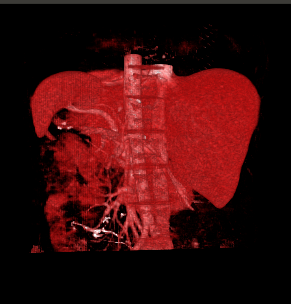
\includegraphics[trim= 0mm 0mm 0mm 0mm, clip, width=1.0\textwidth]{image/sl_0_2.png}}
	\end{columns}

	\setcounter{page}{0}
\end{frame}

%%%%%%%%%%%%%%%%%%%%%%%%%%%%%%%%%%%%%%%%%%%%%%%%%%%%%%%%%%%%%%%%%%%%%%%%%%%%%%% Section

\section{Introduction}

	\subsection[Presentation]{Presentation}
		\begin{frame}
			\frametitle{Presentation}			
			\begin{columns}[c]
			\column{25em}
				\begin{enumerate}
					\item Internship from March to July 2011
					\item Image analysis for diagnostic assistance
					\item Previous work: state of the art
					\item Programming language : Python 2.7
 				\end{enumerate}	
				\column{5em}
				\framebox{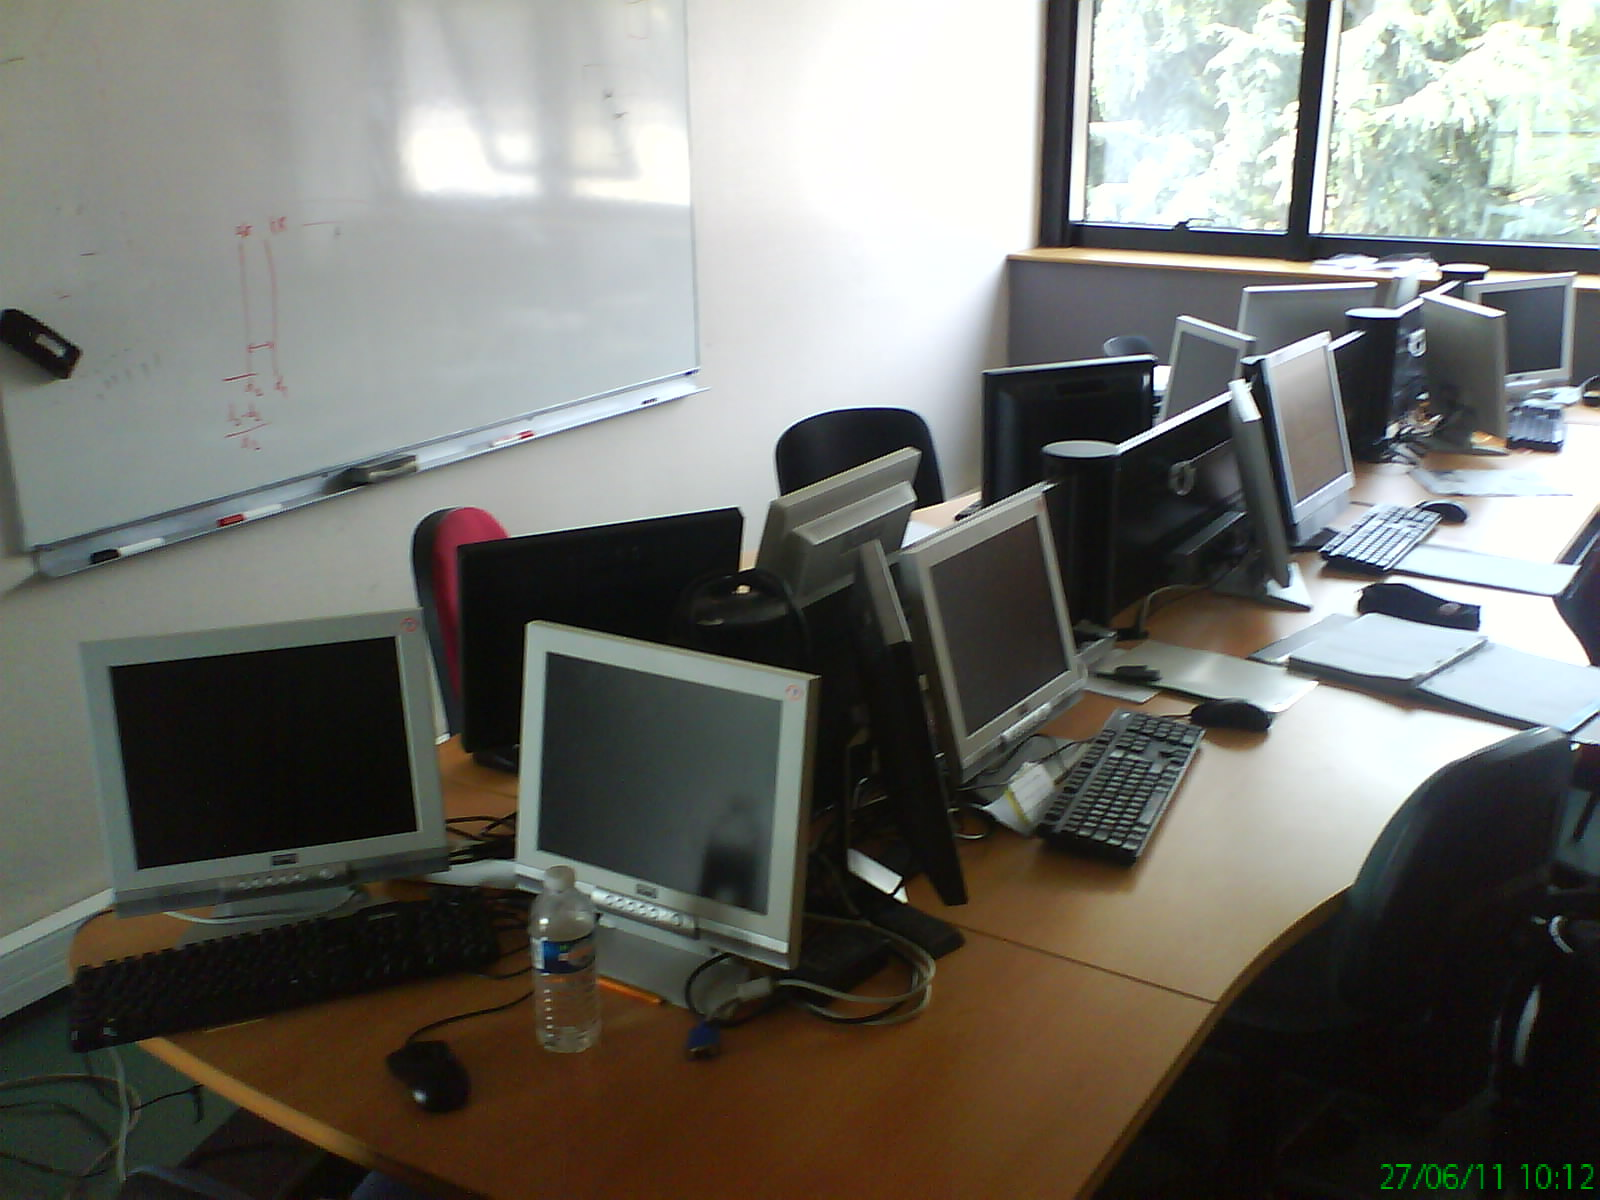
\includegraphics[trim= 0mm 0mm 0mm 0mm, clip, width=1.0\textwidth]{image/lisa_office.JPG}}\vspace{1em}
				\framebox{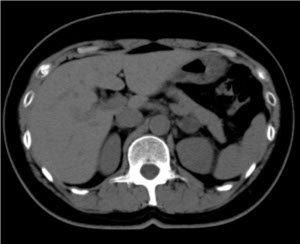
\includegraphics[trim= 0mm 0mm 0mm 0mm, clip, width=1.0\textwidth]{image/image_ct.jpg}}\vspace{1em}		
				\framebox{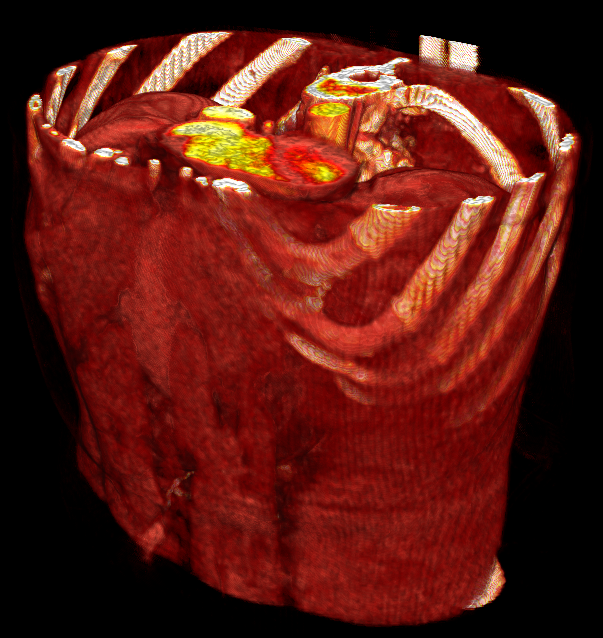
\includegraphics[trim= 0mm 0mm 0mm 0mm, clip, width=1.0\textwidth]{image/body.png}}
			\end{columns}
			\end{frame}

% * * * * * * * * * * * * * * * * * * * * * * * * * * * * * * * * * * * * * * * Slide

	\subsection[Understanding]{Image content understanding}
		\begin{frame}
		\frametitle{Image content understanding : sequential approach}
		%Initial image: 
		%a
		\begin{center}
			\framebox{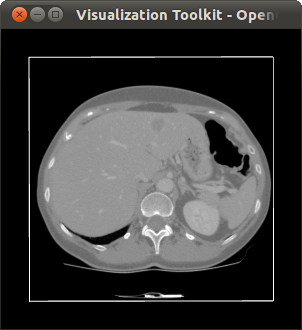
\includegraphics[trim= 10mm 15mm 10mm 28mm, clip, width=0.2\textwidth]{image/int_0_0_0}}\\
%			$\Downarrow$\\
%			\framebox(40,10){Segmentation}\\
			$\swarrow \downarrow \searrow$\\
			\line(1,0){100}\\
			
			\begin{columns}[c]
				\column{6em}
					\begin{center}
						\framebox{
\includegraphics[trim= 15mm 25mm 15mm 35mm, clip, width=1.0\textwidth]{image/int_0_1_2.png}}\vspace{1em}
						\framebox{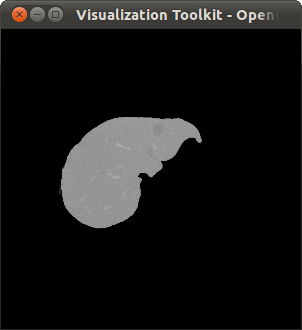
\includegraphics[trim= 15mm 25mm 15mm 35mm, clip, width=1.0\textwidth]{image/int_0_0_2.png}}\\
						$t=1$
					\end{center}
				\column{6em}
				\begin{center}
					\framebox{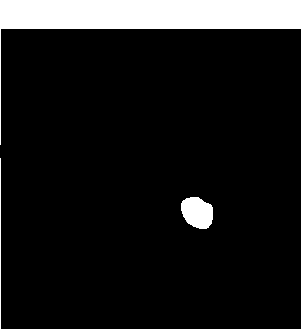
\includegraphics[trim= 15mm 25mm 15mm 35mm, clip, width=1.0\textwidth]{image/int_0_1_3.png}}\vspace{1em}
					\framebox{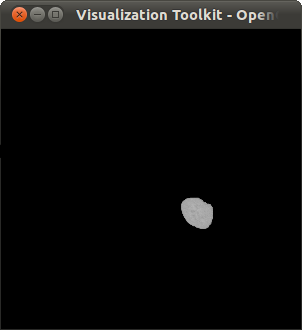
\includegraphics[trim= 15mm 25mm 15mm 35mm, clip, width=1.0\textwidth]{image/int_0_0_3.png}}\\
					$t=2$
				\end{center}
				\column{6em}
				\begin{center}
					\framebox{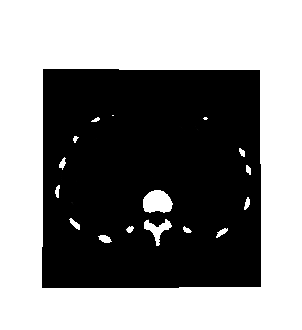
\includegraphics[trim= 15mm 25mm 15mm 35mm, clip, width=1.0\textwidth]{image/int_0_1_4.png}}\vspace{1em}
					\framebox{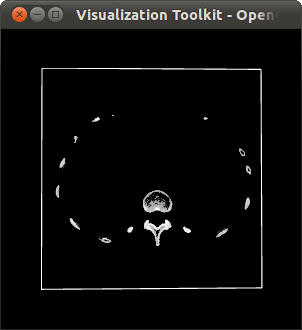
\includegraphics[trim= 15mm 25mm 15mm 35mm, clip, width=1.0\textwidth]{image/int_0_0_4.png}}\\
					$t=3$
				\end{center}
				\column{6em}
				\begin{center}
					\framebox{
\includegraphics[trim= 15mm 24mm 15mm 35mm, clip, width=1.0\textwidth]{image/int_0_1_6.png}}\vspace{1em}
					\framebox{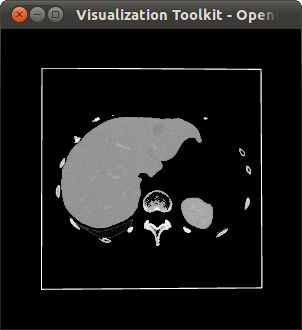
\includegraphics[trim= 15mm 24mm 15mm 35mm, clip, width=1.0\textwidth]{image/int_0_0_6.png}}\\
					%\framebox{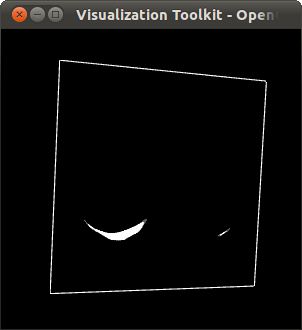
\includegraphics[trim= 20mm 25mm 20mm 35mm, clip, width=1.0\textwidth]{image/int_0_0_5.png}}\\
					Union
				\end{center}
			\end{columns}
			%$\searrow \downarrow \swarrow $	\\		
			%Final image: \framebox{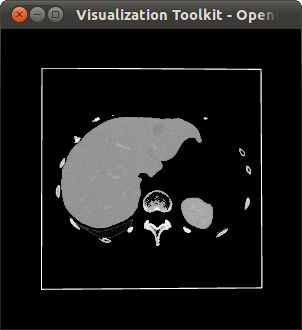
\includegraphics[trim= 15mm 20mm 15mm 30mm, clip, width=0.25\textwidth]{image/int_0_0_6.png}}
		\end{center}			
		
		\end{frame}
		
% * * * * * * * * * * * * * * * * * * * * * * * * * * * * * * * * * * * * * * * Slide

	\subsection[Problem]{Problem statement}
		\begin{frame}
		\frametitle{Problem statement}

%		\begin{columns}[c]
%		\column{25em}
			\begin{block}{How to represent and use non quantitative informations for image content understanding?}
				\begin{enumerate}
					\item e.g. vessels are not included in bones $\Rightarrow$ topology
					\item e.g. vessels are more bright than liver $\Rightarrow$ photometry
				\end{enumerate}

			\end{block}
%		\column{10em}
%			\framebox{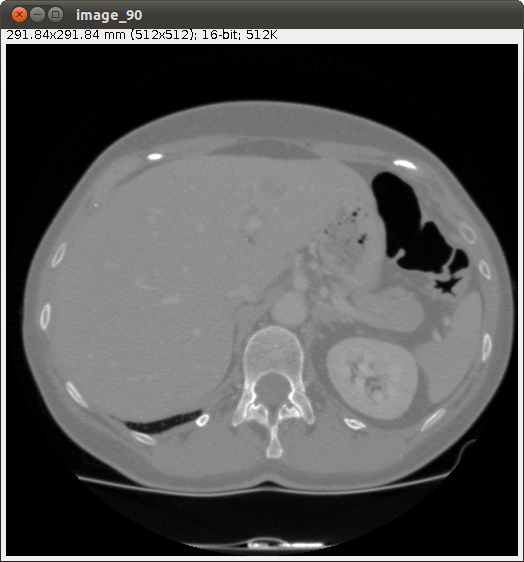
\includegraphics[trim= 5mm 15mm 3mm 25mm, clip, height=0.6\textwidth]{image/dicom.png}}
%		\end{columns}
		
		\vspace{1em}	
		
		\begin{columns}[c]
		\column{10em}
			\framebox{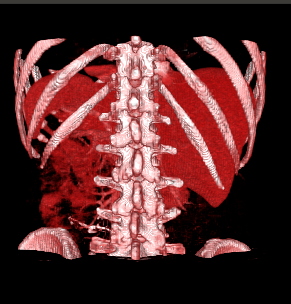
\includegraphics[trim= 0mm 0mm 0mm 0mm, clip, width=1.0\textwidth]{image/sl_0_1.png}}\vspace{1em}
			\framebox{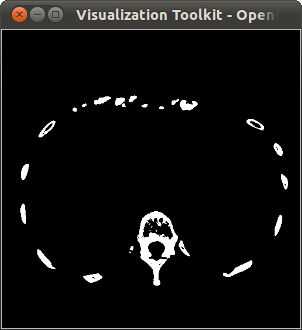
\includegraphics[trim= 0mm 0mm 0mm 20mm, clip, width=0.5\textwidth]{image/mask_bone}}
			\column{0.1em}
			$\Rightarrow$
			\column{10em}
			\framebox{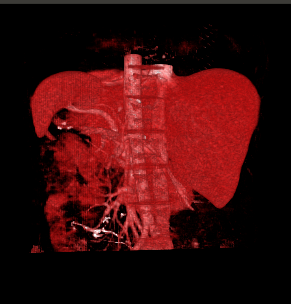
\includegraphics[trim= 0mm 0mm 0mm 0mm, clip, width=1.0\textwidth]{image/sl_0_2.png}}\vspace{1em}
			\framebox{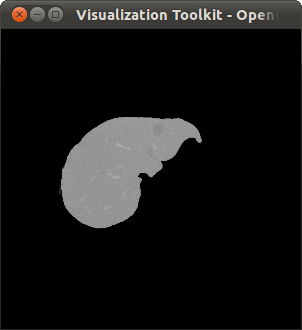
\includegraphics[trim= 10mm 10mm 10mm 30mm, clip, width=0.5\textwidth]{image/int_0_0_2}}			
			\column{0.1em}
			$\Rightarrow$
			\column{10em}
			\framebox{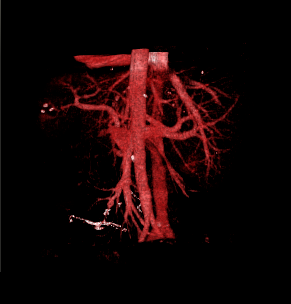
\includegraphics[trim= 0mm 0mm 0mm 0mm, clip, width=1.0\textwidth]{image/sl_0_3.png}}\vspace{6.5em}
		\end{columns}

		\end{frame}

% * * * * * * * * * * * * * * * * * * * * * * * * * * * * * * * * * * * * * * * Slide

	\subsection[State of the art]{State of the art}
		\begin{frame}
		\frametitle{What about state of the art?}
		
		\begin{block}{Image interpretation with a priori conceptual knowledges}

				Example : topological (e.g A include B), relative distance (e.g. A close to B), relative position (e.g. A is left to B)
%					\begin{enumerate}
%						\item[-] Topological (e.g A include B), relative distance (e.g. A close to B), relative position (e.g. A is left to B)
%					\end{enumerate}
			\begin{enumerate}
				\item Not common in image interpretation
				\item Nature
				\begin{enumerate}
					\item[-] Quantitative (e.g. distance, intensity)\footnotemark[1]
					\item[-] Non quantitative (e.g. inclusion, intersection)\footnotemark[2]
				\end{enumerate}
				\item Representation as graph\footnotemark[3]
				\begin{enumerate}
					\item[-] Contextual addition : active node\footnotemark[2]		%	Quantitative (e.g. distance, intensity)\footnotemark[1]
%					\item[-] Non quantitative (e.g. inclusion, intersection)\footnotemark[2]
%				\end{enumerate}				
%				\item Contextual addition
%				\begin{enumerate}
%					\item[-] Principle of active node\footnotemark[2]		
%					%\item[-] Non quantitative (e.g. inclusion, covering) \cite[Fasquel - 2006]{Fasquel2006}
				\end{enumerate}				
%				\item Conceptual graph representation\cite{deruyver2009}
			\end{enumerate}
			
		\end{block}
		
		 \footnotetext[1]{ \tiny \cite{Hudelot2008} C. Hudelot, J. Atif, and I. Bloch, Fuzzy spatial relation ontology for image interpretation, \emph{Fuzzy Sets and Systems}, 2008}
		 \footnotetext[2]{ \tiny \cite{Fasquel2006} J.-B. Fasquel, V. Agnus, An interactive medical image segmentation system based on the optimal management of regions of interest, \emph{Computer Methods and Programs in Biomedicine}, 2006}
		 \footnotetext[3]{ \tiny \cite{deruyver2009} A. Deruyver, Y. Hodéb, and L. Brun, Image interpretation with a conceptual graph, \emph{Artificial Intelligence}, 2009}
		
%		\begin{block}{Contextual information}
%			\begin{enumerate}
%				\item Adaptavive and specific to the image
%				\item Principle of active node \cite[Fasquel - 2006]{Fasquel2006}		
%			\end{enumerate}
%		\end{block}
		
		\begin{alertblock}{Contribution}
			Sequential approach with topological and photometrical knowledges.
		\end{alertblock}\vspace{1em}

%		\begin{columns}[c]		
%		\column{10em}
%			\framebox{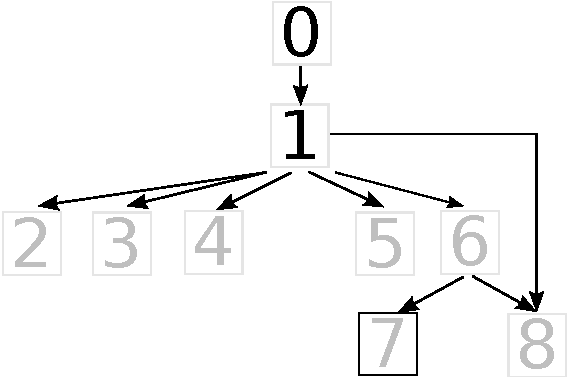
\includegraphics[trim= 0mm 0mm 0mm 0mm, clip, width=0.5\textwidth]{image/im_1_1_gt_0_tumor.pdf}}
%			\column{0.1em}
%			\column{10em}
%			\framebox{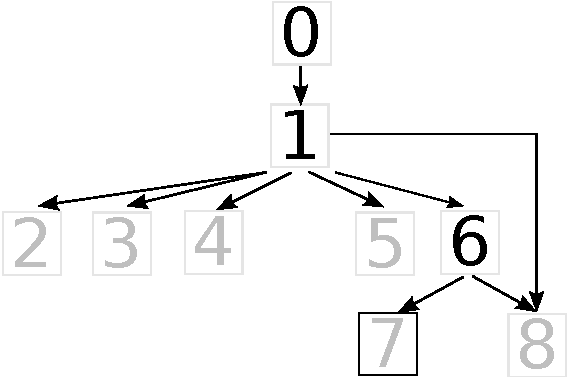
\includegraphics[trim= 0mm 0mm 0mm 0mm, clip, width=0.5\textwidth]{image/im_1_1_gt_1_tumor.pdf}}
%			\column{0.1em}
%			\column{10em}
%			\framebox{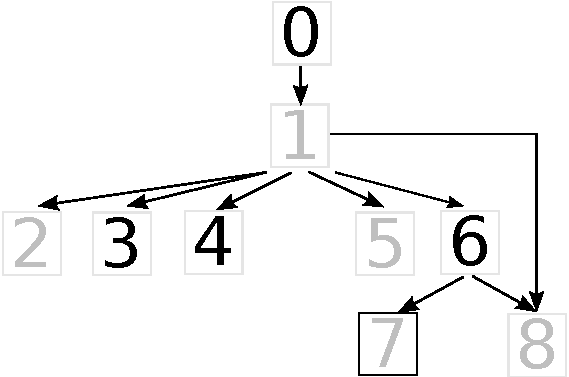
\includegraphics[trim= 0mm 0mm 0mm 0mm, clip, width=0.5\textwidth]{image/im_1_1_gt_2_tumor.pdf}}
%		\end{columns}


		
		\end{frame}

% * * * * * * * * * * * * * * * * * * * * * * * * * * * * * * * * * * * * * * * Slide

	\subsection[Steps]{Steps}	% Il est difficile de relier des informations de haut niveau et de bas niveau
		\begin{frame}
			\frametitle{Steps}
					\begin{columns}[c]
						\column{24em}
							\begin{block}{Representation}
								\begin{enumerate}
									\item Knowledge (conceptual information)
									\item Segmentation process (contextual information)
								\end{enumerate}		
							\end{block}							
							\begin{block}{Formalization (inference engine)}
								\begin{enumerate}
									\item Region of interest (topology)
									\item Number of classes (photometry)
									\item Class ordering (photometry)
								\end{enumerate}		
							\end{block}											
%							\begin{block}{Image}
%								\begin{enumerate}
%									\item Masking, clustering, windowing
%								\end{enumerate}		
%							\end{block}																
						
					\end{columns}

						\begin{columns}[c]
						\column{17em}				
							\begin{alertblock}{Evaluation}
								\begin{enumerate}
									\item Synthetic images
									\item Clustering algorithm
									\item Method's benefits quantification
								\end{enumerate}	
							\end{alertblock}																							
						\column{17em}				
							\begin{alertblock}{Application}
								\begin{enumerate}
									\item Medical images						
									\item Cluster identification
									\item Windowing for volume rendering
								\end{enumerate}	
							\end{alertblock}																							
					\end{columns}
%					\vspace{3em}
%						\alert{Validation from synthetic images to medical images. \\ADD FIGURE OF FULL PROCESS??}
												

						
%							\begin{block}{To do list}
%								\begin{enumerate}
%									\item Representation of conceptual informations
%									\item Modeling of thresholding process
%									\item Formalization of inference engine
%									\item Setting of thresholding algorithms
%								\end{enumerate}		
%							\end{block}



		\end{frame}

%%%%%%%%%%%%%%%%%%%%%%%%%%%%%%%%%%%%%%%%%%%%%%%%%%%%%%%%%%%%%%%%%%%%%%%%%%%%%%% Section

\section{Knowledge representation}
	\subsection[Topology \& photometry]{Topology \& photometry}
	\begin{frame}
		\frametitle{Topology \& photometry (conceptual informations)}
		\begin{block}{Graph}
			%Graphical representation of topologic and photometric relations between all the regions of an image :
			\begin{enumerate}
				\item Nodes are regions (e.g 0, 1, A, B, liver, tumor)
				\item Edges are relations (e.g. include, less bright than)
			\end{enumerate}					
		\end{block}
		\begin{columns}[c]
			\column{10em}		
				\begin{center}
					\framebox{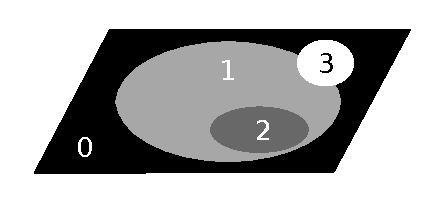
\includegraphics[trim= 0mm 0mm 0mm 0mm, clip, width=1.0\textwidth]{image/abc_img.pdf}}\\
				\end{center}	

			\column{10em}	
				\begin{exampleblock}{Topology}
					\begin{center}
						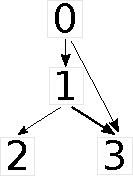
\includegraphics[trim= 0mm 0mm 0mm 0mm, clip, height=0.6\textwidth]{image/abc_graph_topo.pdf}
					\end{center}
				\end{exampleblock}
			\column{10em}
				\begin{exampleblock}{Photometry}
				\begin{center}
					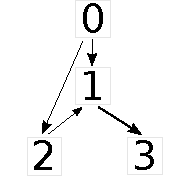
\includegraphics[trim= 0mm 0mm 0mm 0mm, clip, height=0.6\textwidth]{image/abc_graph_photo.pdf}
					\vspace{1em}
					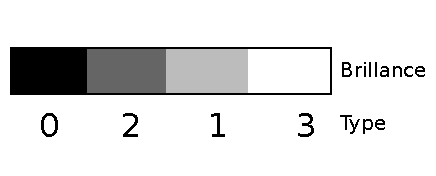
\includegraphics[trim= 0mm 0mm 17mm 0mm, clip, height=0.3\textwidth]{image/abc_graph_photo_gradient.pdf}
				\end{center}

				\end{exampleblock}
					
		\end{columns}	
	\end{frame}
	
% * * * * * * * * * * * * * * * * * * * * * * * * * * * * * * * * * * * * * * * Slide

\subsection[Segmentation process]{Segmentation process}
	\begin{frame}
		\frametitle{Segmentation process modeling (contextual informations)}
		\begin{block}{Add contextual information to the previous graph}
					\begin{enumerate}
						\item Active node = type is segmented
						\item Non active node = type is not segmented
					\end{enumerate}					
				\end{block}	
		\begin{columns}[c]
		
			\column{6em}<1->			
				\begin{exampleblock}{Date $t=0$}
					\begin{center}	
						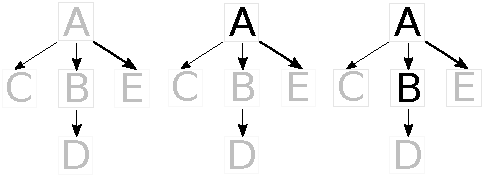
\includegraphics[trim= 0mm 0mm 57mm 0mm, clip, height=0.7\textwidth]{image/contex_gt.pdf}	\vspace{1em}
						
\includegraphics[trim= 0mm 0mm 0mm 0mm, clip, height=0.7\textwidth]{image/me_1_3_img_5.png}	\\
						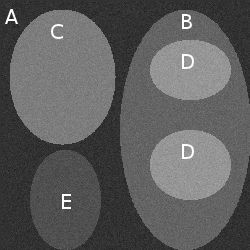
\includegraphics[trim= 0mm 0mm 0mm 0mm, clip, height=0.7\textwidth]{image/me_1_3_img_0.png}						
					\end{center}
				\end{exampleblock}
			\column{0.1em}<2->		
				A\\		
				$\Rightarrow$
			\column{6em}
				\begin{exampleblock}{Date $t=1$}<2->
					\begin{center}
						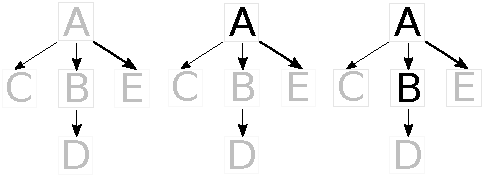
\includegraphics[trim= 28mm 0mm 28mm 0mm, clip, height=0.7\textwidth]{image/contex_gt.pdf}	\vspace{1em}
						
\includegraphics[trim= 0mm 0mm 0mm 0mm, clip, height=0.7\textwidth]{image/me_1_3_img_6.png}	\\%\vspace{1em}
						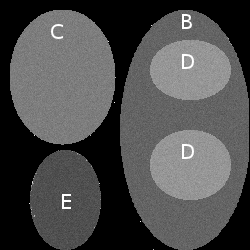
\includegraphics[trim= 0mm 0mm 0mm 0mm, clip, height=0.7\textwidth]{image/me_1_3_img_1.png}						
					\end{center}
				\end{exampleblock}
			\column{0.1em}<3->
				B\\			
				$\Rightarrow$
			\column{6em}
				\begin{exampleblock}{Date $t=2$}<3->
					\begin{center}
						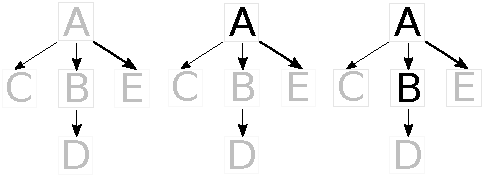
\includegraphics[trim= 56mm 0mm 0mm 0mm, clip, height=0.7\textwidth]{image/contex_gt.pdf}	\vspace{1em}					
						
\includegraphics[trim= 0mm 0mm 0mm 0mm, clip, height=0.7\textwidth]{image/me_1_3_img_7.png}	\\
						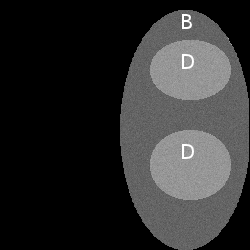
\includegraphics[trim= 0mm 0mm 0mm 0mm, clip, height=0.7\textwidth]{image/me_1_3_img_2.png}						
					\end{center}
				\end{exampleblock}

		\end{columns}
%		\vspace{2em}
%		\alert{Each segmented structure provides a mask that we apply on the original image.}
		
	\end{frame}	
	
%%%%%%%%%%%%%%%%%%%%%%%%%%%%%%%%%%%%%%%%%%%%%%%%%%%%%%%%%%%%%%%%%%%%%%%%%%%%%%% Section

\section[Engine]{Inference engine}
%	\subsection[Presentation]{Presentation}
%	\begin{frame}
%			\frametitle{Presentation}
%			\alert{Mixing conceptual and contextual informations}
%	\end{frame}
	\subsection[ROI]{Region Of Interest}
		\begin{frame}
			\frametitle{From the optimal region of interest...}
			\begin{block}{Optimal Region Of Interest\footnotemark[1]}

				%%%%%%%%%%%%%%%%%%%%%%%%%%%%%%%%%%%%%%%%%%%%%%%%%%%
				\begin{equation}
					R_t(u)=\left(\bigcup_{l\in G_{T,t}^{-1}(u)}X_t(\overline{l})\right) \cup \left(\bigcup_{i\in S_t| u\in G_{T,t}^{-\infty}(i)}X_t(i) \right)
				\end{equation}
				%%%%%%%%%%%%%%%%%%%%%%%%%%%%%%%%%%%%%%%%%%%%%%%%%%%
			\end{block}

			\begin{exampleblock}{Example}
				\begin{columns}[c]
					\column{5em}
					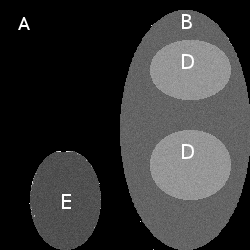
\includegraphics[trim= -5mm 0mm 0mm 0mm, clip, height=1\textwidth]{image/lobe_img.png}
%					\column{5em}
%					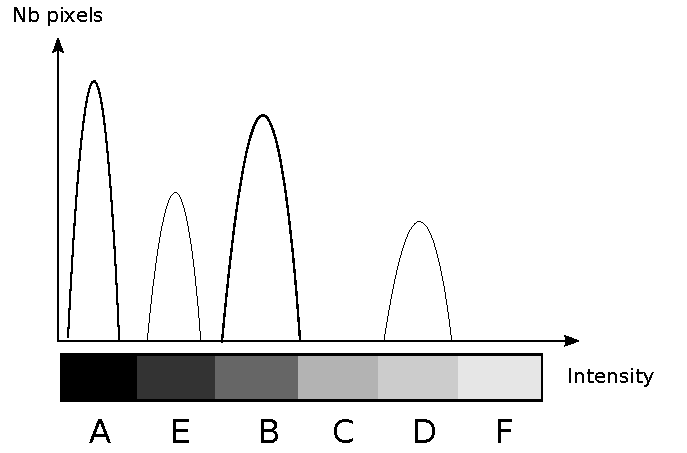
\includegraphics[trim= -5mm 0mm 0mm 0mm, clip, height=1.2\textwidth]{image/lobe_hist.pdf}
					\column{5em}
					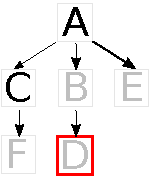
\includegraphics[trim= -5mm 0mm 0mm 0mm, clip, height=1\textwidth]{image/roi_gt.pdf}
				\end{columns}
			\end{exampleblock}

			\begin{columns}[c]	
				\column{15em}			
					\begin{alertblock}{ROI}
						$ R_t(D) = X_t(\bar{A}) $\\
						$ R_t(D) = X_t(A) \setminus X_t(C)$\\
						%$ N_t(D) = 4$

					\end{alertblock}
					
			\end{columns}
		 	\footnotetext[1]{ \cite{Fasquel2006} J.-B. Fasquel, V. Agnus, \emph{Computer Methods and Programs in Biomedicine}, 2006}				
		\end{frame}
		
% * * * * * * * * * * * * * * * * * * * * * * * * * * * * * * * * * * * * * * * Slide

	\subsection[Number of lobes]{Number of classes}
		\begin{frame}
			\frametitle{... to the number of classes}
			\begin{block}{List of classes $\Leftrightarrow$ lobes in the histogram}
				%%%%%%%%%%%%%%%%%%%%%%%%%%%%%%%%%%%%%%%%%%%%%%%%%%%
				\begin{equation}
			 	  	L_t(u) = \Big\{ i \in \left( G_T^{\infty}(G_{T,t}^{-1} (u)) \cap ( S \setminus S_t ) \right) \;|\; \left( G_{T,t}^{-1} (i) \cap G_{T,t}^{-1} (u) \neq \emptyset \right) \Big\} \cup  G_{T,t}^{-1}(u)
				\end{equation}
			 	%%%%%%%%%%%%%%%%%%%%%%%%%%%%%%%%%%%%%%%%%%%%%%%%%%%
			\end{block}			

			\begin{exampleblock}{Example}
				\begin{columns}[c]
					\column{5em}
					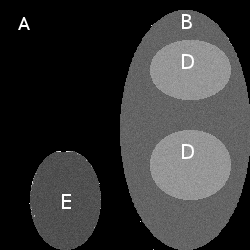
\includegraphics[trim= -5mm 0mm 0mm 0mm, clip, height=1\textwidth]{image/lobe_img.png}
					\column{5em}
					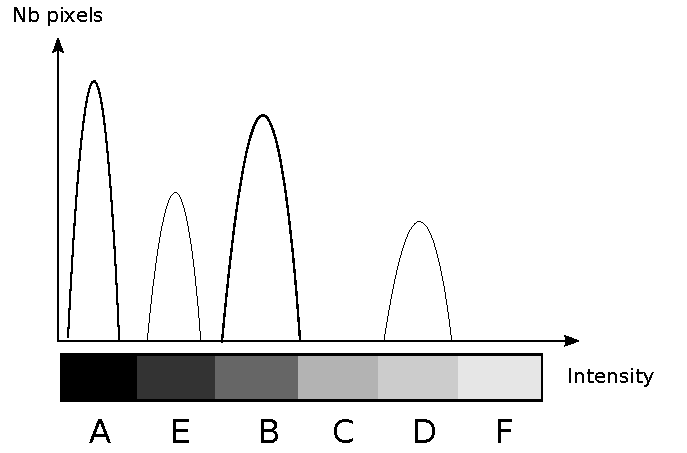
\includegraphics[trim= -5mm 0mm 0mm 0mm, clip, height=1.2\textwidth]{image/lobe_hist.pdf}
					\column{5em}
					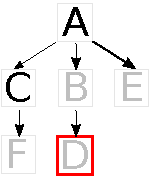
\includegraphics[trim= -5mm 0mm 0mm 0mm, clip, height=1\textwidth]{image/roi_gt.pdf}
%					\column{5em}
%					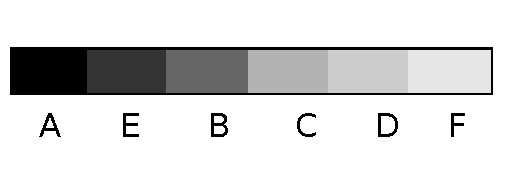
\includegraphics[trim= 0mm 0mm 0mm 0mm, clip, width=1\textwidth]{image/ident_gp.pdf}
					%\hspace{3em}$L_t(D) = \big\{ B, E, D$\hspace{1.35em}| \hspace{5.5em} $\emptyset$\hspace{4.em}\big\}\;$ \cup \;\;\;A$\\
					%\hspace{3em}$L_t(D) = A,B,E,D$
				\end{columns}
			\end{exampleblock}

			\begin{columns}[c]	
				\column{18em}			

				\begin{alertblock}{Cardinality}
					A priori number of classes in the ROI:
					$ N_t(u) = \left|{L_t(u)}\right|$\\
					$ N_t(D) = \left|{L_t(D)}\right| = \left|{B,E,D,A}\right|$\\
					$ N_t(D) = 4$

				\end{alertblock}
				
%				\begin{center}	
%					\framebox{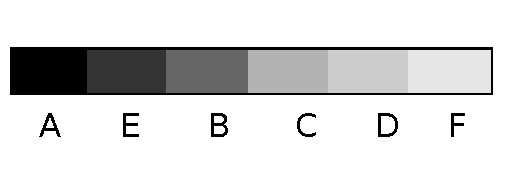
\includegraphics[trim= 0mm 0mm 0mm 0mm, clip, height=0.2\textwidth]{image/ident_gp.pdf}}
%				\end{center}

				\column{15em}	
				\begin{alertblock}{Identification}
				Ordering by photometry: % and \alert{identification}:
				$O_t(u) = \operatorname{ord} \{ L_t(u) \}$
				%$O_t(D) = \operatorname{ord} \{ L_t(D) \}$
				$O_t(D) = \operatorname{ord} \{ B,E,D,A \}$
				$O_t(D) = \{ A, E, B, D \}$
				
				\end{alertblock}					
			\end{columns}


		\end{frame}
		

% * * * * * * * * * * * * * * * * * * * * * * * * * * * * * * * * * * * * * * * Slide

	\subsection[Results]{Results}
		\begin{frame}
			\frametitle{Results}
			\begin{block}{Conclusion}
				\begin{enumerate}
					\item Not easy as it seems
					\item Limit of the study for the number of classes
					\begin{enumerate}
						\item[-] Segmentation of a type in once $\Rightarrow$ no multiplicity
						\item[-] Types are all in the image $\Rightarrow$ no optionality
						%\item Total inclusion (e.g. )
					\end{enumerate}

				\end{enumerate}
			\end{block}			
		\end{frame}
		


		
% * * * * * * * * * * * * * * * * * * * * * * * * * * * * * * * * * * * * * * * Slide


% * * * * * * * * * * * * * * * * * * * * * * * * * * * * * * * * * * * * * * *
% * * * * * * * * * * * * * * * * * * * * * * * * * * * * * * * * * * * * * * *	


	%%clear;bibtex main.aux; pdflatex main.tex ; evince main.pdf &

%Vous préparerez un exposé de 25 minutes qui sera suivi d'une séance de questions.
%Au cours de l'exposé vous devrez :
%1. Formuler un rappel bibliographique et la problématique qui vous a été proposée. -> problem statement + bilio
%2. Présenter les solutions explorées, et les solutions proposées. -> to do list + explanations
%3. Préciser l'originalité de votre travail par rapport à l'existant. Mix photo + topo -> 3D -> liver -> histo -> threshold -> ident -> vessel
%4. Montrer les résultats obtenus et préciser votre apport. -> quantitative analysis
%5. Préciser les publications envisagées. -> possible


% * * * * * * * * * * * * * * * * * * * * * * * * * * * * * * * * * * * * * * * Slide

\section[Evaluation]{Evaluation}


\subsection[Presentation]{Presentation}
	\begin{frame}
	\frametitle{Presentation}
		\center \alert{Which evaluation protocol?}
		\begin{block}{Difficulties}
			\begin{enumerate}
				\item Choice of the clustering algorithm
				\item Procedure (contextual information)
				\item Data (e.g. noise, brightness, region)
			\end{enumerate}		
		\end{block}\vspace{1em}

		\begin{alertblock}{Evaluation}
			\begin{enumerate}
				\item \emph{K-Means} clustering	% Reduction of polluting data : improving efficiency
				\item Synthetic images % Reduction of data volume : CPU time saving
				\item Benefits of knowledge %Algorithm parameterization 
				\begin{enumerate}
					\item[-] Reduction of polluting data and volume
					\item[-] \emph{K-Means} parameterization 
					%\item[-] Number of cluster
					%\item[-] Centroid
				\end{enumerate}
				%\item Class ordering : algorithm parameterization 
			\end{enumerate}		
		\end{alertblock}

%		\begin{columns}[c]	
%			\column{15em}	
%				
%			\column{15em}
%				\begin{exampleblock}{Expected benefits}
%					\begin{enumerate}
%						\item Increasing of useful data percentage
%						\item Processing time saving
%						\item Setting of thresholding algorithms
%						\item Fewer iterations during the segmentation
%					\end{enumerate}		
%				\end{exampleblock}
%		\end{columns}
	\end{frame}


% * * * * * * * * * * * * * * * * * * * * * * * * * * * * * * * * * * * * * * * Slide

	\subsection[Clustering]{Clustering algorithm}
		\begin{frame}
			\frametitle{Clustering algorithm}	
			\setbeamercovered{invisible}		
			\begin{center}
				\alert{Study limited to only one clustering algorithm to illustrate each benefits.}	
			\end{center}
			\begin{block}{K-Means}
				\begin{enumerate}
					\item A widely used clustering algorithm \textit{``the simplicity and computational speed of the K-means algorithm [...] has made it a popular choice''}\footnotemark[1]
					\item Initialization parameters ($k$, centroid) \textit{``the algorithm needs initializing values which greatly influence its terminating optimal solution ... good initialization is crucial for finding globally optimal partitionings''} \footnotemark[1]
				\end{enumerate}
			\end{block}
			\pause
			\begin{columns}[c]	
			\column{3em}
				\framebox{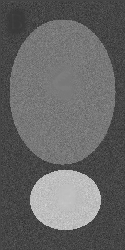
\includegraphics[trim= 0mm 0mm 0mm 0mm, clip, width=1.0\textwidth]{image/me_4_img_2_no_label.png}}
				\column{0.1em}
				$\Rightarrow$
				\column{8em}
				\multiinclude[format=png,graphics={scale=0.2}]{image/me_4_hist_1}\vspace{1em}
				\column{0.1em}
				$\Rightarrow$
				\column{8em}
				\framebox{\includegraphics[trim= 0mm 0mm 0mm 0mm, clip, height=0.9\textwidth]{image/me_4_0_point.png}}		
			\end{columns}			
%			\begin{center}
%					\alert{Number of classes from inference engine = 3}
%			\end{center}
			\footnotetext[1]{ \tiny \cite{Ranjan2010} Anna D. Peterson Ranjan Maitra and Arka P. Ghosh.
, A systematic evaluation of different methods for initializing the k-means clustering algorithm, \emph{Computer Methods and Programs in Biomedicine}, 2010 }
		\end{frame}
				
% * * * * * * * * * * * * * * * * * * * * * * * * * * * * * * * * * * * * * * * Slide

	\subsection[Polluted data]{Reduction of polluting data and volume}
		\begin{frame}
		\frametitle{ROI + number of classes $\Rightarrow$ reduction of polluting data and volume}
  		%\setbeamercovered{dynamic}
		\setbeamercovered{invisible}

		\begin{columns}[c]	
		\column{9em}
			\framebox{\includegraphics[trim= 0mm 0mm 0mm 0mm, clip, height=1.0\textwidth]{image/me_1_0_img_1.png}}\\
			\begin{center}
				4 classes
			\end{center}				
			\column{0.1em}
			$\Rightarrow$
			\column{12em}
			\multiinclude[format=png,graphics={scale=0.2}]{image/me_1_0_hist_1}\vspace{1em}
			\column{0.1em}
			D
			$\Rightarrow$
			\column{9em}
			\framebox{\includegraphics[trim= 0mm 0mm 0mm 0mm, clip, height=1.0\textwidth]{image/me_1_0_bin_1.png}}		
		\end{columns}\vspace{1em}
		\pause
		\begin{columns}[c]	
		\column{9em}
			\begin{center}		
				\framebox{\includegraphics[trim= 0mm 0mm 0mm 0mm, clip, height=1.0\textwidth]{image/me_1_0_img_2.png}}\\
				2 classes
			\end{center}				
			\column{0.1em}
			$\Rightarrow$
			\column{12em}
			\multiinclude[format=png,graphics={scale=0.2}]{image/me_1_0_hist_2}
			\column{0.1em}
			D
			$\Rightarrow$
			\column{9em}
			\begin{center}					
				\framebox{\includegraphics[trim= 0mm 0mm 0mm 0mm, clip, height=1.0\textwidth]{image/me_1_0_bin_2.png}}			
			\end{center}			
		\end{columns}
		\begin{center}
			\alert{ROI improve efficiency and save time.}
		\end{center}

	\end{frame}
	
% * * * * * * * * * * * * * * * * * * * * * * * * * * * * * * * * * * * * * * * Slide

	\subsection[Number of classes]{Number of classes}

		\begin{frame}
		\frametitle{Number of classes $\Rightarrow$ K-Means parameterization}
		\begin{exampleblock}{No a priori number of clusters\footnotemark[1]}
		
		\begin{columns}[c]	
			\column{18em}
				\begin{center}
					\includegraphics[trim= 0mm 0mm 0mm 0mm, clip, width=0.8\textwidth]{image/me_3_3in1_1.pdf}
				\end{center}
			\column{18em}
				\begin{center}		
					\includegraphics[trim= 0mm 44mm 0mm 0mm, clip, width=0.8\textwidth]{image/me_3_3in1.pdf}
				\end{center}					
		\end{columns}\vspace{1em}
		
		\end{exampleblock}
		
		\begin{exampleblock}{A priori number of cluster}
		
		\begin{columns}[c]	
			\column{14em}	
			\begin{enumerate}
				\item Computing time saving
				\item Optimal clustering
			\end{enumerate}			
			\column{18em}
				\begin{center}		
					\includegraphics[trim= 0mm 0mm 0mm 109mm, clip, width=0.8\textwidth]{image/me_3_3in1.pdf}
				\end{center}					
		\end{columns}\vspace{1em}				
		\end{exampleblock}
	\footnotetext[1]{	\tiny \cite[Ray - 1999]{Ray1999} S Ray and R H Turi, Determination of number of clusters in k-means clustering
..., \emph{Advances in Pattern
Recognition and Digital Techniques}, 2007 }
		\end{frame}
	
% * * * * * * * * * * * * * * * * * * * * * * * * * * * * * * * * * * * * * * * Slide

	\subsection[Centroid]{Centroid initialization}
		\begin{frame}
		\frametitle{Number of classes + ordering = centroids $\Rightarrow$ K-Means parameterization}
		\setbeamercovered{invisible}
		\begin{columns}[c]	
			\column{6em}			
				\framebox{\includegraphics[trim= 0mm 0mm 0mm 0mm, clip, width=1.0\textwidth]{image/me_4_img-0.png}}\\
				\hfill 5 classes \hfill \vspace{1em}
				\framebox{\includegraphics[trim= 0mm 0mm 0mm 0mm, clip, width=1.0\textwidth]{image/centroid_gp.pdf}}
				%\multiinclude[format=png,graphics={scale=0.3}]{image/me_4_img}
			\column{3.6em}<2->
				\framebox{\includegraphics[trim= 0mm 0mm 0mm 0mm, clip, width=1.2\textwidth]{image/me_4_img___1.png}}\\
				3 classes
			\column{12em}<2->
				%\multiinclude[format=pdf,graphics={scale=0.3}]{image/me_4_hist}
				\includegraphics[trim= 25mm 0mm 0mm 0mm, clip, height=1.2\textwidth]{image/me_4_hist-1.pdf}
		\end{columns}

		\begin{columns}<3->[c]	
			\column{10em}
				\framebox{\includegraphics[trim= 0mm 0mm 0mm 0mm, clip, height=0.8\textwidth]{image/me_4_point_manual_4_168131.pdf}}
			\column{10em}
				\framebox{\includegraphics[trim= 0mm 0mm 0mm 0mm, clip, height=0.8\textwidth]{image/me_4_point_random_4_168405.pdf}}
			\column{10em}
				\framebox{\includegraphics[trim= 0mm 0mm 0mm 0mm, clip, height=0.8\textwidth]{image/me_4_point_random_3_743240.pdf}}
		\end{columns}	
		\pause\pause
		\begin{center}
			\alert{Careful seeding = better clustering}
		\end{center}
		\end{frame}
		
%%%%%%%%%%%%%%%%%%%%%%%%%%%%%%%%%%%%%%%%%%%%%%%%%%%%%%%%%%%%%%%%%%%%%%%%%%%%%%% Section

\section{Application}
	\subsection[Presentation]{Presentation}
		\begin{frame}
			\frametitle{Presentation}
			\setbeamercovered{invisible}
			%\begin{block}{Inference engine}
				\begin{enumerate}
					\item Visualization only : less restrictive than segmentation
					\item Preliminary results for two use cases
					\item Medical image  from IRCAD\footnote{IRCAD : Institut de Recherche contre les Cancers de l'Appareil Digestif} database (ground truth)
				\end{enumerate}				
			%\end{block}
%			\begin{columns}[c]	
%			\column{8em}			
				\begin{center}
					\multiinclude[format=png,graphics={scale=0.2}]{image/vrrender}\vspace{1em}				
					%\framebox{\includegraphics[trim= 0mm 0mm 0mm 0mm	, clip, height=1\textwidth]{image/body}}\\
%					\framebox{\includegraphics[trim= 10mm 15mm 10mm 28mm, clip, width=1\textwidth]{image/int_0_0_0}}\\
%					\center{$t=0$}\vspace{1em}
%					\framebox{\includegraphics[trim= 10mm 15mm 10mm 35mm, clip, width=1\textwidth]{image/dicom_liver}}\\
%					\center{$t=1$}
%					\framebox{\includegraphics[trim= 20mm 25mm 20mm 35mm, clip, height=0.2\textwidth]{image/int_0_0_3}}
%					\framebox{\includegraphics[trim= 21mm 25mm 19mm 35mm, clip, height=1\textwidth]{image/int_0_0_4}}
				\end{center}
			%\alert{TOPO GRAPH REAL NAME patient>lung,liver + PHOTO GRADIAN}
%			\column{0.1em}
%			\end{columns}					
		\end{frame}
		
		
	\subsection[Context]{Context}
		\begin{frame}
			\frametitle{Context}
			%\setbeamercovered{invisible}
			\begin{columns}[c]	
			\column{8em}			
				\begin{center}
					%\framebox{\includegraphics[trim= 0mm 0mm 0mm 0mm	, clip, height=1\textwidth]{image/body}}\\
					\framebox{\includegraphics[trim= 10mm 15mm 10mm 28mm, clip, width=0.8\textwidth]{image/int_0_0_0}}\\
					\center{$t=0$}\vspace{1em}
					\framebox{\includegraphics[trim= 10mm 15mm 10mm 35mm, clip, width=0.8\textwidth]{image/dicom_liver}}\\
					\center{$t=1$}
%					\framebox{\includegraphics[trim= 20mm 25mm 20mm 35mm, clip, height=0.2\textwidth]{image/int_0_0_3}}
%					\framebox{\includegraphics[trim= 21mm 25mm 19mm 35mm, clip, height=1\textwidth]{image/int_0_0_4}}
				\end{center}
			%\alert{TOPO GRAPH REAL NAME patient>lung,liver + PHOTO GRADIAN}
			\column{0.1em}
				$\Rightarrow$
			\column{17em}			
				\begin{exampleblock}{A priori knowledges}
					\includegraphics[trim= 0mm 0mm 0mm 0mm	, clip, width=1\textwidth]{image/gt_tumor_label}\\
					\includegraphics[trim= 0mm 0mm 0mm 0mm	, clip, width=1\textwidth]{image/gp_tumor_label}
				\end{exampleblock}
				\begin{block}{Inference engine}
					\begin{enumerate}
						\item Number of classes = 3
						\item Ordering = tumor < liver < vessel
					\end{enumerate}				
				\end{block}
%			\column{0.1em}
%				$\Rightarrow$				
%			\column{9em}
%				\begin{block}{Clustering}
%					\begin{enumerate}
%						\item Parameterization
%					\end{enumerate}				
%				\end{block}			
%				\begin{center}
%					\framebox{\includegraphics[trim= 0mm 20mm 0mm 15mm, clip, width=1\textwidth]{image/sl_0_3.png}}\vspace{1em}
%					\framebox{\includegraphics[trim= 0mm 10mm 0mm 15mm, clip, width=1.0\textwidth]{image/im_1_4_tumor_rendering_manual.png}}
%				\end{center}
			\end{columns}					
		\end{frame}

% * * * * * * * * * * * * * * * * * * * * * * * * * * * * * * * * * * * * * * * Slide		
		
%	\subsection[How]{How}
%		\begin{frame}
%			\frametitle{How does it works?}
%			\setbeamercovered{invisible}
%			Example with a medical image :\vspace{1em}
%		\begin{columns}[c]
%			\column{13em}
%				\framebox{\includegraphics[trim= 5mm 10mm 3mm 15mm, clip, height=1.0\textwidth]{image/dicom.png}}	
%				\begin{center}
%	%				\alert{Originality: photometric + topologic informations.}
%					\alert{Can you segment the liver?}
%				\end{center}				
%			\column{13em}
%				\framebox{\includegraphics[trim= 5mm 10mm 3mm 15mm, clip, height=1.0\textwidth]{image/dicom_liver.png}}			
%				\begin{center}
%					\alert{Can you segment the tumors?}
%				\end{center}
%		\end{columns}\vspace{1em}
%		\end{frame}
		
% * * * * * * * * * * * * * * * * * * * * * * * * * * * * * * * * * * * * * * * Slide
	\subsection[Use case : tumor]{Use case : tumor}
		\begin{frame}
			\frametitle{Clustering and windowing for tumor}
			\setbeamercovered{invisible}
		\begin{columns}[c]
			\column{8em}	
				\framebox{\includegraphics[trim= 5mm 0mm 3mm 20mm, clip, width=1\textwidth]{image/liver}}
			\column{20em}			
				\multiinclude[format=png,graphics={scale=0.2}]{image/medical_hist}\vspace{1em}
		\end{columns}\vspace{1em}
	
			\begin{center}
				Windowing for \textcolor{MyGreen}{tumor}
			\end{center}\vspace{1em}
		\begin{columns}[c]
			\column{10em}			
				%\framebox{\includegraphics[trim= 5mm 10mm 3mm 15mm, clip, height=1.0\textwidth]{image/liver.png}}
				\framebox{\includegraphics[trim= 5mm 10mm 3mm 15mm, clip, height=1.0\textwidth]{image/im_1_4_tumor_rendering_kmean.png}}
%			\column{0.1em}
%				$\Rightarrow$
			\column{10em}
				\framebox{\includegraphics[trim= 5mm 10mm 3mm 15mm, clip, height=1.0\textwidth]{image/im_1_4_tumor_rendering_manual.png}}
		\end{columns}\vspace{1em}
			
		\end{frame}		

% * * * * * * * * * * * * * * * * * * * * * * * * * * * * * * * * * * * * * * * Slide

	\subsection[Use case : vessel]{Use case : vessel}
		\begin{frame}
			\frametitle{Clustering and windowing for vessel}
			\setbeamercovered{invisible}
		\begin{columns}[c]
			\column{8em}	
				\vspace{1em}
				\framebox{\includegraphics[trim= 5mm 3mm 0mm 10mm, clip, width=0.9\textwidth]{image/im_3_0_render_all}}
			\column{20em}			
				\includegraphics[trim= 0mm 0mm 0mm 0mm, clip, height=0.45\textwidth]{image/medical_vessel_windowing}
		\end{columns}\vspace{2em}
			\begin{center}
				Windowing for \textcolor{red}{vessel}
			\end{center}\vspace{1em}
		\begin{columns}[c]
			\column{10em}			
				\framebox{\includegraphics[trim= 5mm 10mm 3mm 15mm, clip, height=1.0\textwidth]{image/im_3_0_render_vessel_kmean.png}}
			%\column{8em}
				%\framebox{\includegraphics[trim= 5mm 10mm 3mm 15mm, clip, height=1.0\textwidth]{image/im_3_0_render_vessel_1_sigma.png}}
			\column{10em}
				\framebox{\includegraphics[trim= 5mm 10mm 3mm 15mm, clip, height=1.0\textwidth]{image/im_3_0_render_vessel_manual.png}}
		\end{columns}\vspace{1em}
			
		\end{frame}		
%%%%%%%%%%%%%%%%%%%%%%%%%%%%%%%%%%%%%%%%%%%%%%%%%%%%%%%%%%%%%%%%%%%%%%%%%%%%%%% Section

%\section{Analyse}
%	\begin{frame}
%		\frametitle{frame5}
%	\end{frame}

%%%%%%%%%%%%%%%%%%%%%%%%%%%%%%%%%%%%%%%%%%%%%%%%%%%%%%%%%%%%%%%%%%%%%%%%%%%%%%%% Section

%\section[Perspectives]{Perspectives et ameliorations}
%	\begin{frame}
%		\frametitle{frame5}
%	\end{frame}
	
%%%%%%%%%%%%%%%%%%%%%%%%%%%%%%%%%%%%%%%%%%%%%%%%%%%%%%%%%%%%%%%%%%%%%%%%%%%%%%% Section

\section{Conclusion}
	\begin{frame}
		\frametitle{Conclusion}
		\begin{block}{Results}
			\begin{enumerate}
				\item	Generic method for image understanding
				\item	Non quantitative $\Rightarrow$ adaptability
				\item	Constraints:
				\begin{enumerate}
					\item	Perfectly segmented masks
					\item	Complete graph completion			
				\end{enumerate}
			\end{enumerate}
		\end{block}
		\begin{block}{Refinements}
			\begin{enumerate}
				\item	$N$ type value to handle multiplicity and optionality
				\item	Node fully included by successors
			\end{enumerate}
		\end{block}
%		\begin{block}{Prospect}
%			\begin{enumerate}
%				\item	Perfectly segmented masks
%				\item	Graph completion				
%				%\item	
%			\end{enumerate}
%		\end{block}
		
		\begin{block}{Personal}
			\begin{enumerate}
				\item Very pleasant job (research, tools)
				\item Formalization is not easy
				\item The best part just started
			\end{enumerate}
		\end{block}
	\end{frame}


% * * * * * * * * * * * * * * * * * * * * * * * * * * * * * * * * * * * * * * *
% * * * * * * * * * * * * * * * * * * * * * * * * * * * * * * * * * * * * * * *	





\begin{frame}
	\center Work achievement 
	\center Document Analysis Group\vspace{2em}
	\titlepage
	\thispagestyle{empty}
	\begin{center}
		%\includegraphics[height=30mm]{unejolieimage.jpg}
	\end{center}
%	\textit{\small christophe.rigaud@etud.univ-angers.fr}
%	\begin{flushleft}
%		Supervisor: Jean-Baptiste FASQUEL
%	\end{flushleft}	
		\includegraphics[trim= 0mm 0mm 0mm 0mm, clip, width=3em]{image/LogoL3i.png}\hspace{18em}
		\includegraphics[width=3cm]{image/logo_cvc_centrevisio.png}\vspace{1em}

		\tiny	Supervisors: Dimosthenis Karatzas, Joost van de Weijer \hspace{19em}Jean-Christophe Burie, Jean-Marc Ogier 

\end{frame}

% * * * * * * * * * * * * * * * * * * * * * * * * * * * * * * * * * * * * * * * Slide

\begin{frame} 
	\begin{center}{\Large Plan }\end{center}

	\thispagestyle{empty}
	\begin{columns}[c]
		\column{15em}
		\tableofcontents[hideallsubsections]
		\column{15em}
			%\framebox{\includegraphics[trim= 0mm 0mm 0mm 0mm, clip, width=1.0\textwidth]{image/sl_0_2.png}}
	\end{columns}

	\setcounter{page}{0}
\end{frame}

%%%%%%%%%%%%%%%%%%%%%%%%%%%%%%%%%%%%%%%%%%%%%%%%%%%%%%%%%%%%%%%%%%%%%%%%%%%%%%% Section

\section{Introduction}

	\subsection[Context]{Context}
		\begin{frame}
			\frametitle{Context}			
			\begin{columns}[c]
			\column{15em}
				\framebox{\includegraphics[trim= 0 0 0 0, clip, height=1.4\textwidth]{image/ROUDIER_LESTERRESCREUSEES_010.jpg}}
% 				\begin{chronology}[5]{1983}{2010}{3ex}{\textwidth}
% 				\event{1984}{one}
% 				\event[1985]{1986}{two}
% 				\event{\decimaldate{25}{12}{2001}}{three}
% 				\end{chronology}

				\column{15em}
\framebox{\includegraphics[trim= 0 0 0 0, clip, height=1.4\textwidth]{image/MCCAY_LITTLENEMO_001.jpg}}
% 				\framebox{\includegraphics[trim= 0mm 0mm 0mm 0mm, clip, width=1.0\textwidth]{image/lisa_office.JPG}}\vspace{1em}
% 				\framebox{\includegraphics[trim= 0mm 0mm 0mm 0mm, clip, width=1.0\textwidth]{image/image_ct.jpg}}\vspace{1em}		
% 				\framebox{\includegraphics[trim= 0mm 0mm 0mm 0mm, clip, width=1.0\textwidth]{image/body.png}}
			\end{columns}
			\footnotetext[1]{ McCay, Little nemo, \emph{Slumberland}, 1905}
			\footnotetext[2]{ Nicolas Roudier, \emph{Les terres creusées}, 2011}
			\end{frame}

% * * * * * * * * * * * * * * * * * * * * * * * * * * * * * * * * * * * * * * * Slide

	\subsection[Threshold]{Optimal threshold selection}
		\begin{frame}
		\frametitle{Optimal threshold selection}
		%Initial image: 
		\begin{columns}[c]
		\column{10em}
			\framebox{\includegraphics[trim= 600px 20px 500px 400px, clip, width=1\textwidth]{image/bin_50.png}}\vspace{1em}
			%\framebox{\includegraphics[trim= 600px 20px 500px 400px, clip, width=0.5\textwidth]{image/mask_bone}}
			\column{0.1em}
			$\Rightarrow$
			\column{10em}
			\framebox{\includegraphics[trim= 600px 20px 500px 400px, clip, width=1.0\textwidth]{image/bin_100.png}}\vspace{1em}
			%\framebox{\includegraphics[trim= 10mm 10mm 10mm 30mm, clip, width=0.5\textwidth]{image/int_0_0_2}}			
			\column{0.1em}
			$\Rightarrow$
			\column{10em}
			\framebox{\includegraphics[trim= 600px 20px 500px 400px, clip, width=1.0\textwidth]{image/bin_200.png}}\vspace{1em}
		\end{columns}
		
		\end{frame}
		
% * * * * * * * * * * * * * * * * * * * * * * * * * * * * * * * * * * * * * * * Slide

	\subsection[Letter1]{Letter extraction 1}
		\begin{frame}
		\frametitle{Letter extraction}

			\begin{block}{Black on white connected components (CC) selection rules}
				\begin{enumerate}
					\item high contrast ratio
					\item no overlapping
					\item surrounded by other CC similar in height
				\end{enumerate}

			\end{block}
		\begin{columns}[c]
			\column{15em}%trim=l b r t  width=0.5\textwidth, 
			  \framebox{\includegraphics[trim= 0 120px 20px 25px, clip, height=0.7\textwidth]{image/bright.png}}\vspace{1em}
			  %\framebox{\includegraphics[trim= 600px 20px 500px 400px, clip, width=0.5\textwidth]{image/mask_bone}}
			\column{15em}
			  \framebox{\includegraphics[trim= 0 120px 20px 25px, clip, height=0.7\textwidth]{image/overlap.png}}\vspace{1em}
		\end{columns}
		
		\end{frame}


% * * * * * * * * * * * * * * * * * * * * * * * * * * * * * * * * * * * * * * * Slide

	\subsection[Letter2]{Letter extraction 2}
		\begin{frame}
		\frametitle{Letter extraction}

			\begin{block}{Black on white connected components (CC) selection rules}
				\begin{enumerate}
					\item high contrast ratio
					\item no overlapping
					\item surrounded by other CC similar in height
				\end{enumerate}

			\end{block}
		\begin{columns}[c]
			\column{15em}%trim=l b r t  width=0.5\textwidth, 
			  \framebox{\includegraphics[trim= 0 120px 20px 25px, clip, height=0.7\textwidth]{image/surroundd.png}}\vspace{1em}
			  %\framebox{\includegraphics[trim= 600px 20px 500px 400px, clip, width=0.5\textwidth]{image/mask_bone}}
			\column{15em} 
			  \framebox{\includegraphics[trim= 0 0px 0px px, clip, height=0.7\textwidth]{image/4_direction.png}}\vspace{1em}
		\end{columns}
		
>		\end{frame}

% * * * * * * * * * * * * * * * * * * * * * * * * * * * * * * * * * * * * * * * Slide

	\subsection[Line]{Letter to lines}
		\begin{frame}
		\frametitle{Letter to lines}
		\begin{center}	
		  \framebox{\includegraphics[trim= 200px 280px 300px 200px, clip, width=0.80\textwidth]{image/letter_position.pdf}}\vspace{1em}
		\end{center}
		
		\begin{block}{Horizontal and vertical alignment}

			\begin{enumerate}
				\item $d<Max(h1,h2)$
				\item $c2_y \in [y1_{min},y1_{max}]$
			\end{enumerate}
			
		\end{block}
		
		
		\end{frame}

% * * * * * * * * * * * * * * * * * * * * * * * * * * * * * * * * * * * * * * * Slide


%%%%%%%%%%%%%%%%%%%%%%%%%%%%%%%%%%%%%%%%%%%%%%%%%%%%%%%%%%%%%%%%%%%%%%%%%%%%%%% Section

\section{Experiments and results}
	\subsection[Dataset]{Dataset}
	\begin{frame}
		\frametitle{Dataset}
		\begin{center}	
		  \framebox{\includegraphics[trim= 0 0 0 0, clip, width=0.90\textwidth]{image/dataset.jpg}}\vspace{1em}
		\end{center}
		\begin{block}{}
			%Graphical representation of topologic and photometric relations between all the regions of an image :
			\begin{enumerate}
				\item Available at http://dagdata/documents/ ``Comics''
				\item 100 pages from 20 different authors
				\item > 5000 text lines
			\end{enumerate}					
		\end{block}
		

	\end{frame}
	
% * * * * * * * * * * * * * * * * * * * * * * * * * * * * * * * * * * * * * * * Slide

	\subsection[Ground truth]{Ground truth}
	\begin{frame}
		\frametitle{Ground truth}
		\begin{center}	
		  \framebox{\includegraphics[trim= 0 0 0 0, clip, width=0.90\textwidth]{image/gt_tool.png}}\vspace{1em}
		\end{center}
		\begin{block}{}
			%Graphical representation of topologic and photometric relations between all the regions of an image :
			\begin{enumerate}
				\item Tool from L3i laboratory (La Rochelle, France)
				\item 20/100 pages
				\item Line level
			\end{enumerate}				
		\end{block}
		

	\end{frame}

% * * * * * * * * * * * * * * * * * * * * * * * * * * * * * * * * * * * * * * * Slide

\subsection[Results]{Results}
	\begin{frame}
		\frametitle{Results}
		\begin{center}	
		  \framebox{\includegraphics[trim= 0 0 0 0, clip, width=0.90\textwidth]{image/evaluation.png}}\vspace{1em}
		\end{center}
		\begin{block}{}
					\begin{enumerate}
						\item ICDAR 2011 Robust Reading Competition - Challenge 1: Reading Text in Born-Digital Images (Web and Email)\footnotemark[1]
					\end{enumerate}					
				\end{block}
		
%		\vspace{2em}
%		\alert{Each segmented structure provides a mask that we apply on the original image.}
		\footnotetext[1]{ D. Karatzas, S. Robles Mestre, J. Mas, F. Nourbakhsh, P. Pratim Roy, \emph{In Proc. 11th International Conference of Document Analysis and Recognition}, 2011}

	\end{frame}	
	
%%%%%%%%%%%%%%%%%%%%%%%%%%%%%%%%%%%%%%%%%%%%%%%%%%%%%%%%%%%%%%%%%%%%%%%%%%%%%%% Section

\section[Conclusion]{Conclusion}
	\subsection[Conclusion]{Conclusion}
	\begin{frame}
			\frametitle{Conclusion & perspectives}

		\begin{columns}[c]
			\column{15em}%trim=l b r t  width=0.5\textwidth, 
			  \begin{block}{Before (1/05/12)}
				  \begin{enumerate}
					  \item Frame + text extraction\footnotemark[1]
					  \item 5 ground truth pages
				  \end{enumerate}
				\end{block}
			\column{15em} 
			  \begin{exampleblock}{After (27/07/12)}
				  \begin{enumerate}
					  \item Improved text extraction
					  \item 20 ground truth pages
					  \item Text validation
					  \item 1 publication (in progress)
					  \item Balloon detection
				  \end{enumerate}
				\end{exampleblock}
		\end{columns}

		  \begin{alertblock}<2>{Thanks!}
				  \begin{enumerate}
					  \item Centre de Visión per Computador
					  \item Document Analysis Group
				  \end{enumerate}
				\end{alertblock}
				
				
	\footnotetext[1]{ Rigaud, C., Tsopze, N., Burie, J.-C., and Ogier, J.-M., Robust frame and text extraction from comic books \emph{Lecture Note for Computer Science
GREC'11}, 2011}
	\end{frame}
% 	\subsection[Balloon]{Balloon detection}
% 		\begin{frame}[hide]
% 			\frametitle{Balloon detection}
% 		\begin{center}	
% 		  \framebox{\includegraphics[trim= 0 0 0 0, clip, width=0.90\textwidth]{image/balloon_real.png}}\vspace{1em}
% 		\end{center}
% 
% 		\footnotetext[1]{ Lubbin, Les bulles du labo, \emph{Episode 5}, 2012}
% 		\end{frame}
		
% * * * * * * * * * * * * * * * * * * * * * * * * * * * * * * * * * * * * * * * Slide




	%\bibliographystyle{plain}							% ordre alphabétique et les numérote en conséquence.
	%\bibliographystyle{unsrt}							% trie les entrées par ordre d’apparition dans le texte.

	%\bibliographystyle{natbib}
	%\bibliography{bibliography}
	%\bibliographystyle{alpha}
	%\bibliography{bibi.bib}
%	\begin{thebibliography}{10}
%		\bibitem{Goldbach1742}[Goldbach, 1742]
%		  Christian Goldbach.
%		  \newblock A problem we should try to solve before the ISPN '43 deadline,
%		  \newblock \emph{Letter to Leonhard Euler}, 1742.
%	\end{thebibliography}

\end{document}

% * * * * * * * * * * * * * * * * * * * * * * * * * * * * * * * * * * * * * * *
% * * * * * * * * * * * * * * * * FIN * * * * * * * * * * * * * * * * * * * * *
% * * * * * * * * * * * * * * * * * * * * * * * * * * * * * * * * * * * * * * *

